\iffalse

%%%%%%%%%%%%%%%%%%%%%%%%%%%%%%%%%%%%%%%%%%%%%%%%%%%%%%%%%%%%%%%%%%%%%%%%
%
% This is the template file for the 6th International conference
% NONLINEAR ANALYSIS AND EXTREMAL PROBLEMS
% June 25-30, 2018
% Irkutsk, Russia
%
%%%%%%%%%%%%%%%%%%%%%%%%%%%%%%%%%%%%%%%%%%%%%%%%%%%%%%%%%%%%%%%%%%%%%%%%
% The preparation of the article is based on the standard llncs class
% (Lecture Notes in Computer Sciences), which is adjusted with style
% file of the conference.
%
% There are two ways of compilation of the file into PDF
% 1. Use pdfLaTeX (pdflatex), (LaTeX+DVIPS will not work);
% 2. Use LuaLaTeX (XeLaTeX will work too).
% When using LuaLaTeX You will need TTF or OTF CMU fonts
% (Computer Modern Unicode). The fonts are installed with 'cm-unicode' package in
% a distribution of LaTeX % (https://www.ctan.org/tex-archive/fonts/cm-unicode),
% either by downloading and installing these fonts system wide, the address of their page is
% http://canopus.iacp.dvo.ru/%7Epanov/cm-unicode/
% The second option won't work in XeLaTeX.
%
% For MiKTeX (LaTeX distribution for Windows),
%  1. Package 'cm-unicode' is installed manually with the MiKTeX administration Console.
%  2. For the compilation of this example, namely, the stub figure, one will also need to
% download package 'pgf' manually. This package uses in the popular
% package tikz.
%  3. Tests showed that the rest of the required packages MiKTeX loads automatically (if
%     it is allowed). The 'auto download' option is
%     configured in 'Settings' section in MiKTeX Console.
%
%
% The easiest way to compile an article is to use pdfLaTeX, but
% the final layout of the book will be compiled with LuaLaTeX,
% as a result will be of better quality thanks to the package 'microtype' and
% use vector OTF instead of standard raster fonts of pdfLaTeX.
%
% In the case of questions and problems with the article compilation,
% write letters to e-mail: eugeneai@irnok.net, Cherkashin Evgeny.
%
% New version of the correcting style file will be available at the website:
%     https://github.com/eugeneai/nla-style
%     file - nla.sty
%
% Further instructions are in the text body of the template. The template itself
% is an article example.
%
% The LaTeX2e format is used!

% 12 points font size is used.
\documentclass[12pt]{llncs}

% The correcting style file is added.
\usepackage{todonotes}

\usepackage{nla} % This package is needed for compiling
                 % this template, it should be removed
                 % from your article.

% Many popular packages (amsXXX, graphicx, etc.) are already imported in the style file.
% If there is a conflict with your packages, try disabling them and compile
% the text.
%
% It would be convenient in the layout of the proceedings if the file names
% of the figures of different authors do not clash.
% To minimize the clash, the drawings can be placed in a separate subfolder
% named after the author or the title of the paper.
%
% \graphicspath{{ivanov-petrov-pics/}} % specifies the folder with images in png, pdf formats.
% or
% \graphicspath{{great-problem-solving-paper-pics/}}.

\begin{document}

% Text should be formatted in accordance with the 'article' class, using extensions like
% AMS.
%
\fi
\title{The Modified Monowave Method \\for the Reachable Set Approximation of \\the Nonlinear Controlled System on the Plane
	%\thanks{The research is supported by RFBR (RNF, other funds), project No.~00-00-00000.}
}
% First author
\author{Tatiana Zarodnyuk%\inst{1}
  \and
  Alexander Gornov%\inst{2}
%  \and
%  Name FamilyName3\inst{1}
}
\institute{Matrosov Institute for System Dynamics and Control Theory of SB RAS, Irkutsk, Russia\\
  \email{tzarodnyuk@gmail.com, gornov@icc.ru}
 % \and
%Affiliation, City, Country\\
%\email{email@example.com}
}
% etc

\maketitle

\begin{abstract}
The paper deals with the monowave method allowed to construct the boundary of the reachable set for controlled dynamical system. It is presented the results of numerical experiments for nonconvex optimal control test problems.

\keywords{controlled dynamical system, monowave method, reachable set}
\end{abstract}
% at the end of the list, there should be no final dot
%\section{The main results}
We propose the numerical technique based on the approximation of the reachable set boundary for controlled dynamical system. The presented monowave method uses the given sequence of the control functions with a variable switching point. To build ''the wave'' of the control function, the time interval is divided into equal parts. Then we construct the control functions as relay functions with the switching point selected at the nodes of the resulting grid. 

To study the computational properties of the proposed method, the series of computational experiments have been carried out. Test examples are presented in which it was possible to simply set the boundary of the reachable set,  it is impossible to recreate the boundaries correctly, and examples in which the construction of the boundary of the reachable set deteriorates with an increase in the time interval. 

It is found that too few points may not be enough to construct the boundary of the reachable set. As the number of points increases, the boundary of the set can be built better (Fig.~\ref{zzfig:example}).

% The figures and tables are drawn according to the standard class 'article'.
\begin{figure}[htb]
  \centering

% Two picture formats are supported:
%\includegraphics[width=0.7\linewidth]{figure.pdf} % Raster format
%\includegraphics[width=0.7\linewidth]{figure.png} % Vector and raster format
%
% Vector drawings can be drawn in Inkscape editor
% https://inkscape.org/ru/download/
% The usual format of the editor is SVG, so the drawings must be exported in
% PDF or PNG (with a resolution of minimum 150 dpi, and maximum of 300 dpi).
   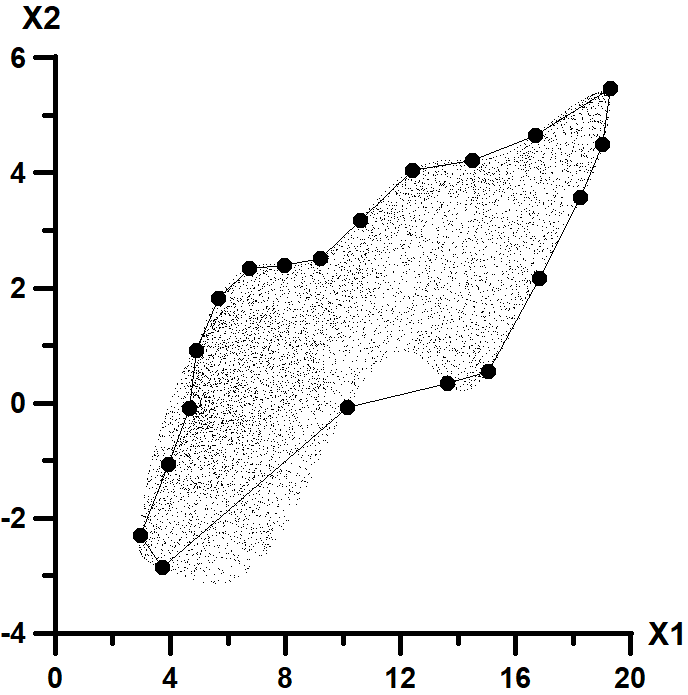
\includegraphics[width=0.29\linewidth]{zarodnyuk_fig01.png}
   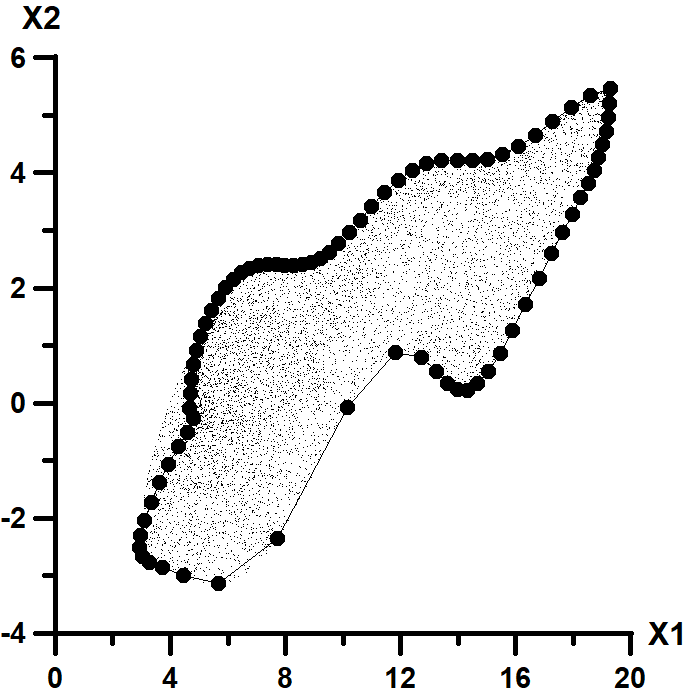
\includegraphics[width=0.29\linewidth]{zarodnyuk_fig02.png}
   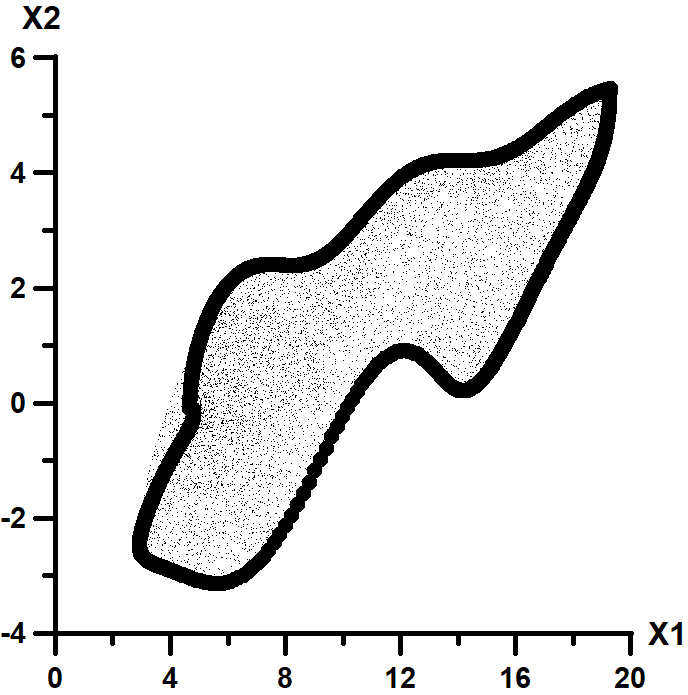
\includegraphics[width=0.29\linewidth]{zarodnyuk_fig03.png}
   \caption{The well-known reachable set for the optimal control problem of the nonlinear pendulum oscillations \cite{Pub1}}\label{zzfig:example}
\end{figure}

% At the end of the text, acknowledgments are expressed, if you haven't
% made a footnote from the title. For example, we can write
%The research is carried on with support of RFBR (RNF, other funds), project No.~00-00-00000.

\begin{thebibliography}{9} % or {99}, if there is more than ten references.
\bibitem{Pub1} Gornov A.Y., Zarodnyuk T.S., Madzhara T.I., Daneyeva A.V., Veyalko I.A. A collection of test multiextremal optimal control problems. Springer Optimization and Its Applications.~2013. Vol.~76. Pp.~257--274.

\end{thebibliography}
%\end{document}

%%% Local Variables:
%%% mode: latex
%%% TeX-master: t
%%% End:
